\documentclass[10pt,twocolumn]{article}
\usepackage[utf8]{inputenc}
\usepackage[T1]{fontenc}
\usepackage{lmodern}
\usepackage[margin=0.85in]{geometry}
\usepackage{amsmath,amssymb,booktabs,graphicx,microtype}
\usepackage[hidelinks]{hyperref}
\newcommand{\E}{\mathbb{E}}

\title{\textbf{What Reward Alone Can and Cannot Fix:\\ REINFORCE Fine-Tuning of a 344K-Parameter Language Model}}
\author{Melih Akbulut}
\date{November 2026}

\begin{document}
\maketitle

\begin{abstract}
We study reinforcement-learning (RL) fine-tuning of language models in the smallest setting we could
build that still shows the interesting phenomena: a 344K-parameter character-level transformer,
three algorithmic tasks (multi-digit addition, string reversal, digit sorting), and plain REINFORCE
with a binary reward from an automatic verifier. The model is pretrained by maximum likelihood on a
corpus in which hard task instances are rare (2\%), then fine-tuned on hard instances using reward
only, with no gold answers. Across three seeds, RL raises hard-instance exact match from
37.1\% to 96.9\% on sorting and from 84.6\% to 100\% on reversal, close to supervised fine-tuning
with gold labels (99.3\% and 100\%), while forgetting far less of the easy regime (easy addition
drops to 92.2\% under RL versus 62.2\% under supervised fine-tuning). RL does nothing for hard
addition, where the pretrained model succeeds on only 0.3\% of prompts: reward-only learning amplified
competence that was already present and did not create it. We also document a failure mode: at a
higher learning rate, two of three runs collapse abruptly to 0\% on every task, and a KL penalty
toward the pretrained model prevents this at the cost of slower improvement. A variance-reducing
baseline and a shaped partial-credit reward, two standard ingredients, made no measurable difference
here. Every experiment runs in about ten minutes on one CPU core.
\end{abstract}

\noindent\textbf{Özet (Turkish abstract).}
{\small 344 bin parametreli, karakter düzeyinde küçük bir transformer dil modelini önce denetimli
olarak ön-eğitiyor, ardından yalnızca otomatik bir doğrulayıcıdan gelen 0/1 ödülle (doğru cevaplar
gösterilmeden) REINFORCE kullanarak zor görev örneklerinde iyileştiriyoruz. Üç seed üzerinde
pekiştirmeli öğrenme, zor sıralama görevinde tam eşleşmeyi \%37,1'den \%96,9'a, zor ters çevirmede
\%84,6'dan \%100'e çıkarıyor; bu, etiketli ince ayara (\%99,3 ve \%100) yakın ve kolay görevlerde
çok daha az unutmayla gerçekleşiyor. Buna karşın ön-eğitimli modelin neredeyse hiç başaramadığı zor
toplama görevinde (\%0,3) hiçbir iyileşme olmuyor: ödül, var olan yetkinliği güçlendiriyor ama
sıfırdan yetkinlik üretmiyor. Yüksek öğrenme oranında üç koşudan ikisi aniden çöküyor; ön-eğitimli
modele doğru bir KL cezası bunu önlüyor.}

\section{Introduction}
Fine-tuning language models with reinforcement learning is now routine, from preference-based
tuning~\cite{ouyang2022} to verifier-rewarded training of reasoning models~\cite{shao2024,guo2025}.
These systems are expensive to study: one run costs many GPU-hours, so ablations and repeated seeds
are rare. This paper asks how much of the qualitative behaviour of RL fine-tuning can be reproduced
in a model small enough to train on a laptop CPU in minutes, where every claim can be checked over
several seeds.

Our setting mirrors the large-scale recipe in miniature. A language model is first pretrained with
maximum likelihood on a corpus that covers a task distribution unevenly: easy instances are common
and hard ones are rare. It is then improved on the hard instances by sampling answers, scoring them
with an automatic verifier, and applying the policy gradient. No gold answers are used in the second
stage.

We report four findings.
\begin{enumerate}
\itemsep0pt
\item \textbf{Reward-only fine-tuning works when the model sometimes succeeds.} Hard sorting goes
from 37.1\% to 96.9\% and hard reversal from 84.6\% to 100\%, close to supervised fine-tuning.
\item \textbf{It fails when the model almost never succeeds.} Hard addition stays at 0.3\%.
\item \textbf{RL forgot less than supervised fine-tuning.} Easy-addition accuracy fell by 4 points
under RL and by 34 points under supervised fine-tuning on the same hard distribution.
\item \textbf{Unregularised REINFORCE can collapse.} At a three times larger learning rate, two of
three runs fall to 0\% on all tasks; a KL anchor to the pretrained model prevents it.
\end{enumerate}
We also report two negative ablation results: neither a moving-average baseline nor a shaped reward
changed the outcome.

\section{Setup}
\paragraph{Tasks.} Sequences are character strings over a 28-token vocabulary (digits, letters
\texttt{a}--\texttt{j}, \texttt{+ = :}, three task tags, end-of-sequence and padding). Three tasks
share one model:
\begin{itemize}
\itemsep0pt
\item \emph{Addition}: \texttt{A:607+4818=} $\to$ \texttt{5425}, most significant digit first.
\item \emph{Reversal}: \texttt{R:dheagib=} $\to$ \texttt{bigaehd}.
\item \emph{Sorting}: \texttt{S:439150=} $\to$ \texttt{013459}.
\end{itemize}
Each task has an \emph{easy} regime (operands of 1--2 digits; strings of length 2--5) and a
\emph{hard} regime (operands of 3--4 digits; strings of length 6--9).

\paragraph{Model.} A decoder-only transformer~\cite{vaswani2017} with 3 layers, width 96, 4 heads,
learned absolute positions and a context of 28 tokens: 343{,}776 parameters.

\paragraph{Stage 1: pretraining.} Maximum likelihood on answer tokens for 2{,}500 steps of batch
size 128 (AdamW, learning rate $10^{-3}$). Each example is drawn from a uniformly chosen task and is
hard with probability 0.02. The resulting model is near-perfect on easy instances and has uneven,
partial competence on hard ones (Table~\ref{tab:main}, first row).

\paragraph{Stage 2: RL fine-tuning.} For each step we draw 128 hard prompts $x$ (tasks uniform),
sample an answer $y \sim \pi_\theta(\cdot\mid x)$ of at most 10 tokens, and obtain a reward
$r(x,y)=\mathbf{1}[y=y^\star(x)]$ from a verifier. We minimise
\begin{multline*}
\mathcal{L}(\theta) = -\E\big[(r - b_{\tau})\log \pi_\theta(y\mid x)\big] \\
 + \beta\,\E\big[\mathrm{KL}\big(\pi_\theta(\cdot\mid x,y_{<t})\,\|\,\pi_{0}(\cdot\mid x,y_{<t})\big)\big],
\end{multline*}
the REINFORCE estimator~\cite{williams1992} with a per-task exponential-moving-average baseline
$b_\tau$ (decay 0.9) and a per-token KL penalty toward the frozen pretrained model
$\pi_0$~\cite{jaques2017}, evaluated on the sampled trajectories. The default uses $\beta=0.1$,
AdamW with learning rate $10^{-4}$, gradient clipping at 1.0, and 1{,}500 steps (192{,}000 episodes).

\paragraph{Reference and ablations.} \emph{SFT} is supervised fine-tuning on the same hard
distribution with gold answers, the same optimiser and the same number of examples; it uses
information RL does not have and serves as a reference, not a competitor. Ablations remove the
baseline, remove the KL term, replace the binary reward with a shaped one (1 for an exact match,
otherwise half the fraction of positions that match), train on sorting only, and raise the learning
rate to $3\times10^{-4}$ with $\beta\in\{0,1\}$.

\paragraph{Evaluation.} Greedy decoding, exact match, on 500 fixed prompts per task and regime
drawn from the same generators with a separate seed. Every configuration is run from three
independently pretrained models; we report mean $\pm$ standard deviation over those three seeds.

\begin{table*}[t]
\centering\small
\begin{tabular}{lcccccc}
\toprule
 & \multicolumn{3}{c}{Easy regime (not trained in stage 2)} & \multicolumn{3}{c}{Hard regime (stage-2 target)} \\
\cmidrule(lr){2-4}\cmidrule(lr){5-7}
Method & Add & Reverse & Sort & Add & Reverse & Sort \\
\midrule
\csname @@input\endcsname table_main.tex
\bottomrule
\end{tabular}
\caption{Greedy exact-match accuracy (\%) after stage 2, mean $\pm$ std over 3 seeds, 500 test
prompts per cell. ``RL, sort only'' receives reward for hard sorting alone. With learning rate
$3\times10^{-4}$ and no KL term, two of the three seeds collapsed to 0\% on every task, which is
what the large standard deviations in that row reflect.}
\label{tab:main}
\end{table*}

\begin{figure*}[t]
\centering
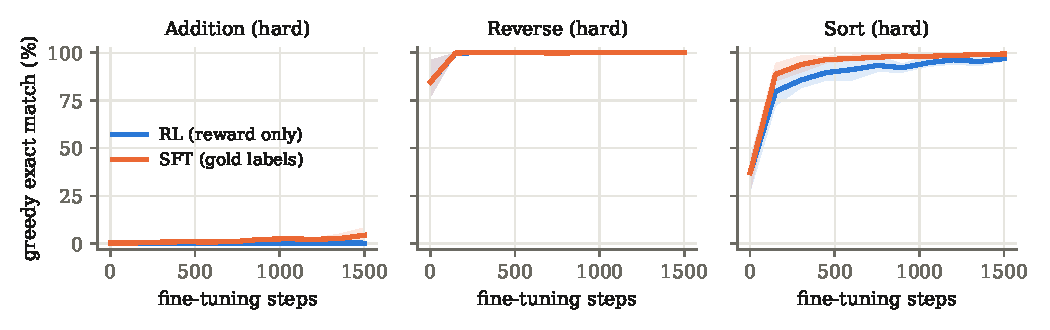
\includegraphics[width=0.92\textwidth]{fig_curves.pdf}
\caption{Hard-regime accuracy during stage 2 for RL (binary reward, no labels) and SFT (gold
labels). Lines are the mean over 3 seeds; bands span the minimum and maximum.}
\label{fig:curves}
\end{figure*}

\begin{figure*}[t]
\centering
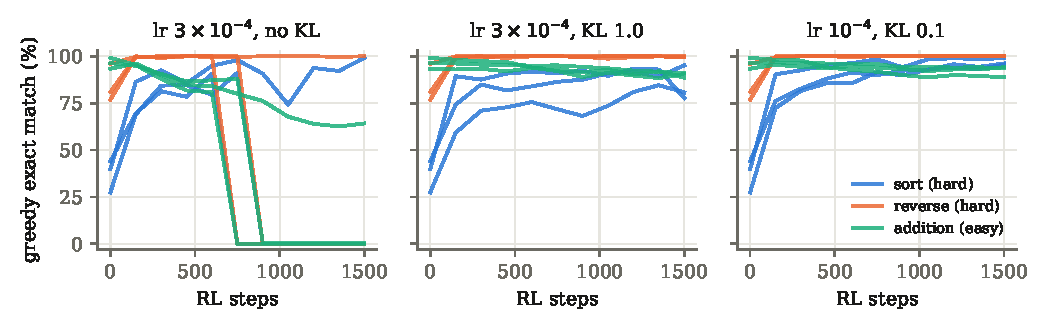
\includegraphics[width=0.92\textwidth]{fig_stability.pdf}
\caption{Per-seed training curves (one line per seed and metric). Left: without a KL anchor at the
higher learning rate, two of three runs collapse on all tasks between steps 600 and 900 and do not
recover. Middle: a strong anchor removes the collapse but slows the gain on sorting. Right: the
default configuration.}
\label{fig:stability}
\end{figure*}

\section{Results}
\paragraph{RL closes most of the gap on tasks with partial competence.}
Table~\ref{tab:main} and Figure~\ref{fig:curves} show the main comparison. On hard sorting RL moves
the model from 37.1\% to 96.9\%, against 99.3\% for SFT; on hard reversal both reach 100\%. Most of
the gain arrives in the first 150 steps. RL trails SFT slightly throughout on sorting, which is
expected: a label carries more information per example than one bit of reward.

\paragraph{RL does not help where the starting success rate is near zero.}
On hard addition the pretrained models answer 0.3\% of test prompts correctly and RL leaves this
unchanged. With a binary reward, an episode contributes a non-zero learning signal only when a
sampled answer is exactly right, so there is almost nothing to reinforce. The shaped reward, which
pays for partially correct answers, did not change this (0.6\%). SFT, which is told the answer, reaches
only 4.4\% in the same budget, so this task is hard for the model at this size and training
length regardless of the signal; the experiment shows that RL did not overcome the cold start, and
does not show how much of the difficulty is specific to RL.

\paragraph{RL forgot less than SFT.}
Neither method sees easy instances in stage 2. Under SFT, easy addition falls from 96.3\% to 62.2\%
and easy sorting from 97.6\% to 91.4\%. Under RL, easy addition falls to 92.2\% and easy sorting
does not fall. The KL anchor accounts for little of this: without it RL still retains 89.7\% on easy
addition. We did not test the cause. One explanation consistent with the data is that SFT applies
large gradients on hard addition, which it cannot yet solve and which shares its task tag with easy
addition, while RL receives almost no gradient there because the reward is almost always zero.

\paragraph{Training on one task damages the others.}
Rewarding only hard sorting brings it to 99.1\%, but hard reversal drops from 84.6\% to 73.9\% and
easy addition from 96.3\% to 84.9\%, even with the KL anchor (which is applied only on sorting
prompts in this run). Multi-task reward avoided this.

\paragraph{Collapse and the KL anchor.}
At learning rate $3\times10^{-4}$ without a KL term, two of three runs improve for 600--750 steps
and then drop to 0\% on all six test sets within one evaluation interval, without recovery
(Figure~\ref{fig:stability}, left). In an earlier trial run with the same failure, the collapsed
model had stopped emitting the end-of-sequence token and produced maximum-length strings. With
$\beta=1$ all three runs are stable, but hard sorting reaches only 84.6\%. At learning rate
$10^{-4}$ no run collapsed with or without the anchor, so in this setting the anchor matters as
insurance against an aggressive step size; it was not needed for the default configuration.

\paragraph{Baseline and reward shaping made no measurable difference.}
Removing the baseline gave 99.5\% on hard sorting against 96.9\% with it, and the shaped reward
gave 97.0\%. With three seeds and standard deviations of 0.3--1.6 points we do not read the
2.6-point advantage of the no-baseline variant as established, but there is clearly no benefit from
the baseline. With a non-negative binary reward and no baseline, the update is a likelihood step on
the model's own correct samples, which is a low-variance signal when success is frequent.

\section{Related work}
REINFORCE~\cite{williams1992} was applied to sequence generation to optimise non-differentiable
metrics, starting from a likelihood-pretrained model~\cite{ranzato2016}, often with a baseline given
by the model's own greedy output~\cite{rennie2017}. Penalising divergence from the pretrained model
during RL was introduced for sequence models by Jaques et al.~\cite{jaques2017} and is standard in
preference-based tuning of large models~\cite{ouyang2022}, typically together with
PPO~\cite{schulman2017}. Verifier-rewarded training on mathematical and reasoning tasks at scale is
described in~\cite{shao2024,guo2025}. Small transformers trained on arithmetic are a common testbed
for studying learning dynamics~\cite{lee2024}. Our contribution is not a new method but a minimal,
fully reproducible setting in which the benefits and failure modes of this recipe can be measured
across seeds.

\section{Limitations}
The model, tasks and budgets are tiny, and nothing here shows that the same effects hold at scale.
All results use three seeds, which is enough to see the large effects (the sorting gain, the
forgetting gap, the collapse) and not enough to rank the ablations that differ by a few points.
Hyperparameters were chosen from a small trial sweep on seed 0, and the test prompts are drawn from
the same generators as the training prompts without removing overlaps, which matters little for the
hard regime (the space of prompts is large) but means easy-regime numbers measure retention and not
generalisation. We tested one RL algorithm; PPO-style clipping, larger batches or a curriculum from
easy to hard instances might change the cold-start result on addition, and we did not try them. The
explanations offered for the forgetting gap and for the collapse are hypotheses that the experiments
do not test.

\section{Conclusion}
In a 344K-parameter language model, plain REINFORCE with a binary verifier reward recovered almost
all of the benefit of supervised fine-tuning on tasks the model could already solve some of the
time, forgot less of what it was not trained on, and was useless on a task it could not yet solve at
all. A KL anchor to the pretrained model guarded against an abrupt collapse at a higher learning
rate. The code trains everything from scratch on one CPU core in about ten minutes per run, which
makes this a convenient setting for testing ideas about RL fine-tuning before spending GPU time on
them.

\paragraph{Reproducibility.} All code is in \texttt{tinyrl.py} (model, tasks, training),
\texttt{run\_all.sh} (experiment grid) and \texttt{analyze.py} (table and figures). Wall-clock time
on one CPU core: about 6 minutes for pretraining, 10 for an RL run and 4 for an SFT run.

\begin{thebibliography}{9}
\small
\bibitem{williams1992} R.~J. Williams. Simple statistical gradient-following algorithms for
connectionist reinforcement learning. \emph{Machine Learning}, 8(3--4):229--256, 1992.
\bibitem{vaswani2017} A.~Vaswani et al. Attention is all you need. \emph{NeurIPS}, 2017.
\bibitem{ranzato2016} M.~Ranzato, S.~Chopra, M.~Auli, W.~Zaremba. Sequence level training with
recurrent neural networks. \emph{ICLR}, 2016.
\bibitem{rennie2017} S.~Rennie et al. Self-critical sequence training for image captioning.
\emph{CVPR}, 2017.
\bibitem{jaques2017} N.~Jaques et al. Sequence Tutor: Conservative fine-tuning of sequence
generation models with KL-control. \emph{ICML}, 2017.
\bibitem{schulman2017} J.~Schulman et al. Proximal policy optimization algorithms.
\emph{arXiv:1707.06347}, 2017.
\bibitem{ouyang2022} L.~Ouyang et al. Training language models to follow instructions with human
feedback. \emph{NeurIPS}, 2022.
\bibitem{shao2024} Z.~Shao et al. DeepSeekMath: Pushing the limits of mathematical reasoning in
open language models. \emph{arXiv:2402.03300}, 2024.
\bibitem{guo2025} D.~Guo et al. DeepSeek-R1: Incentivizing reasoning capability in LLMs via
reinforcement learning. \emph{Nature}, 645:633--638, 2025.
\bibitem{lee2024} N.~Lee et al. Teaching arithmetic to small transformers. \emph{ICLR}, 2024.
\end{thebibliography}
\end{document}
